% !TEX root = main.tex
%
% Preamble for the IJM final report.  Document class is the University
% of Warsaw bachelor-thesis class (pracamgr.cls), the same class used by
% the Rift / Duckling LS reference thesis: clean title page, proper
% chapters, and alpha-style citations.
\documentclass[licencjacka,en]{pracamgr}

%-- Encoding / fonts -------------------------------------------------------
\usepackage[utf8]{inputenc}
\usepackage[T1]{fontenc}
% Use the default Computer Modern family (same as the Duckling LS thesis).
% No \usepackage{times} -- CM looks better at thesis sizes.

%-- Math -------------------------------------------------------------------
\usepackage{amsmath}
\usepackage{amssymb}

%-- Floats / figures -------------------------------------------------------
\usepackage{graphicx}
\usepackage[dvipsnames, table]{xcolor}
\usepackage{float}
\usepackage{rotating}
\usepackage{caption}
\usepackage{subcaption}

%-- Tables -----------------------------------------------------------------
\usepackage{tabu}
\usepackage{tabularx}
\usepackage{ltablex}
\usepackage{longtable}
\usepackage{xltabular}
\usepackage{booktabs}

%-- UML sequence diagrams --------------------------------------------------
\usepackage{pgf-umlsd}
\usepackage{tikz}
\usetikzlibrary{positioning, arrows.meta, calc, patterns, backgrounds}

%-- Misc -------------------------------------------------------------------
\usepackage{wasysym}
\usepackage{pifont}
\usepackage{ifthen}
\usepackage{xspace}
\usepackage{enumitem}
\usepackage{soul}

\newcommand{\supported}{\ding{52}\xspace}
\newcommand{\unsupported}{\ding{55}\xspace}
\newcommand{\partsupported}{\textcolor{black!40}{\ding{52}}\xspace}
\newcommand{\lowsupported}{\textcolor{black!20}{\ding{52}}\xspace}
\newcommand{\unknowsupported}{\textbf{?}\xspace}

\newcommand{\authors}{Jan Wangrat}
\newcommand{\professor}{Prof.~Danilo Ardagna,\\ Ph.D.~Candidate Federica Filippini}
\newcommand{\projectName}{Intelligent Job Management}

%-- Microtype --------------------------------------------------------------
\usepackage[protrusion=true]{microtype}

%-- Tight typography -------------------------------------------------------
\sloppy
\emergencystretch=6em
\tolerance=2000
\hbadness=10000
\vbadness=10000
\hfuzz=3pt

% Match the Duckling LS thesis: black serif headings on a clean report
% layout, no Polimi-blue accents.  We keep titlesec only for the tighter
% spacing -- the visual style is the report class default.
\usepackage{titlesec}
\titleformat{\chapter}[hang]
  {\normalfont\huge\bfseries}{\thechapter.}{0.6em}{}
\titlespacing*{\chapter}{0pt}{-15pt}{18pt}
\titleformat{\section}
  {\normalfont\Large\bfseries}{\thesection}{0.6em}{}
\titlespacing*{\section}{0pt}{14pt}{6pt}
\titleformat{\subsection}
  {\normalfont\large\bfseries}{\thesubsection}{0.6em}{}
\titlespacing*{\subsection}{0pt}{10pt}{4pt}
\titleformat{\subsubsection}
  {\normalfont\normalsize\bfseries}{\thesubsubsection}{0.6em}{}
\titlespacing*{\subsubsection}{0pt}{8pt}{3pt}

%-- Captions ---------------------------------------------------------------
% Match the Duckling LS look: small justified caption text, bold label.
\captionsetup{font=small,labelfont=bf,format=plain,
              justification=justified}

%-- Listings ---------------------------------------------------------------
\usepackage{listings}
\definecolor{lstback}{rgb}{0.96,0.96,0.92}
\definecolor{lstcomment}{rgb}{0,0.5,0}
\definecolor{lstkey}{rgb}{0.55,0.10,0.55}
\definecolor{lststring}{rgb}{0.58,0,0.82}
\lstdefinestyle{ijm}{
  backgroundcolor=\color{lstback},
  basicstyle=\footnotesize\ttfamily,
  commentstyle=\color{lstcomment}\itshape,
  keywordstyle=\color{lstkey}\bfseries,
  stringstyle=\color{lststring},
  numberstyle=\tiny\color{Gray},
  breaklines=true,
  breakatwhitespace=true,
  captionpos=b,
  numbers=left,
  numbersep=6pt,
  frame=single,
  framesep=2mm,
  xleftmargin=1.5em,
  showspaces=false,
  showstringspaces=false,
  showtabs=false,
  tabsize=2,
  keepspaces=true,
}
\lstset{style=ijm}

%-- Float placement (prevent huge whitespace from floats jumping pages) ----
\renewcommand{\topfraction}{0.95}
\renewcommand{\bottomfraction}{0.95}
\renewcommand{\textfraction}{0.05}
\renewcommand{\floatpagefraction}{0.85}
\setlength{\textfloatsep}{8pt plus 2pt minus 2pt}
\setlength{\intextsep}{8pt plus 2pt minus 2pt}
\setlength{\dbltextfloatsep}{8pt plus 2pt minus 2pt}

%-- Hyperref ---------------------------------------------------------------
% Loaded by pracamgr.cls; configure quietly -- subtle dark-blue links
% like the Duckling LS thesis, not bright Polimi-blue.
\hypersetup{colorlinks=true,
            linkcolor=black,
            citecolor=black,
            urlcolor=black,
            pdfborder={0 0 0}}

%-- Utilities --------------------------------------------------------------
\input{util/highlight}
\input{util/abbrev}


% Thesis metadata used by \makeOwnTitle (pracamgr.cls).
\autor{Jan Wangrat}{}
\title{Intelligent Job Management}
\kierunek{Computer Science and Engineering}
\opiekun{Prof. Danilo Ardagna\\
  Politecnico di Milano\\
  with Federica Filippini, Ph.D. Candidate}
\date{\today}
\keywords{GPU scheduling, deep learning, job management, profile-aware
optimisation, distributed systems, FastAPI, PostgreSQL, Docker}

\begin{document}
\makeOwnTitle

\begin{abstract}
Intelligent Job Management (IJM) is~a~scheduler for~shared GPU clusters
that combines profile-aware placement, deadline-driven preemption,
and~cross-version checkpoint resume.  It~extends the~ANDREAS project
(Politecnico di~Milano) from a~single-host prototype to~a~distributed
control plane: one FastAPI service drives per-node workers over
SSH-tunnelled HTTP, an~external GPUspb optimiser handles standard-run
placement, and~training jobs migrate between heterogeneous GPU
generations (A40, QuadroP600) without losing progress.  The~report
describes the~deployment topology, the~four-phase scheduling pipeline,
the~configuration surface, and~two end-to-end scenarios that exercise
the~system on~a~two-node cluster.
\end{abstract}

\tableofcontents

\chapter{Introduction}\label{ch:introduction}
Modern deep-learning research depends on shared GPU clusters in which
training jobs compete for a~small number of~expensive accelerators.
Operators are expected to~place each job on~the~hardware that meets its
deadline at~the~lowest cost, despite per-GPU prices that vary by~more
than an~order of~magnitude between generations.  Manual scheduling
quickly becomes the~bottleneck, and~off-the-shelf cluster managers
(Kubernetes, plain SLURM) treat GPU bundles as~interchangeable and~have
no~notion of~per-job energy budgets or~deadline-aware preemption.

The ANDREAS project~\cite{andreas} at~Politecnico di~Milano demonstrated
that a~cost-aware optimiser, fed with~profile measurements of~each job
type on~each hardware bundle, can~plan placements that beat the~typical
operator's intuition.  ANDREAS ran on~the~ARMIDA cluster~--- uniform
Tesla~V100 nodes~--- dispatching containers to~them through SLURM, and~its
implementation is~not~available to~reuse.  The~two-node Polimi cluster
targeted here is~instead \emph{heterogeneous}: an~A40 node alongside
a~legacy QuadroP600 node on~different CUDA and~torch generations.  A~job
preempted on~one node must therefore resume across torch versions when
it~migrates to~the~other, and~the~scheduler must consume a~standalone
optimiser (GPUspb~\cite{filippini2023pathrelinking,filippini2024stochastic})
as~an~HTTP service rather than embed one.

This report describes Intelligent Job~Management (IJM), an~independent
reimplementation of~the~ANDREAS approach as~a~distributed control plane.
The~control plane is~a~single FastAPI service that hosts the~profiling scheduler, the
optimiser client, and~the~per-node slot semaphores.  Each GPU node runs
a~lightweight worker that owns the~local Docker daemon.  The~two are
glued together by~plain HTTP over SSH~tunnels, so the~same code runs on
a~laptop talking to~a~remote cluster and~on~a~single-host development
machine.  IJM integrates the~GPUspb optimiser as~the~external decision
maker for~standard-run placement.  Before any instance is~placed as~a
standard run, the~scheduler first executes a~small number of~profile
runs for~it on~previously-unmeasured (node, GPU-count) cells, so the
optimiser is~never asked to~score an~unmeasured bundle.  Migration between
the~A40 and~legacy P600 nodes mid-training is~what makes such placement
worthwhile, and~it~is~not~free: a~PyTorch checkpoint is~normally locked to
the~version that~wrote it, and~the~two nodes can~only exchange one through
a~shared filesystem.  IJM closes both gaps~--- a~deliberately
version-tolerant checkpoint format and~an~rclone-mounted shared store~---
and~asks of~each training job only that~it~honour a~small
\emph{contract}; the~solution and~its reasoning are~detailed in
\S\ref{sec:checkpoints} and~the~contract in~Chapter~\ref{ch:config}.

We validate IJM with~two end-to-end scenarios on~the~two-node cluster,
each exercising the~full job lifecycle and~checking that the~system
faithfully realises the~optimiser's decisions.  Scenario~1
(under-subscribed) submits five instances of~\texttt{cnn\_big}, a
compute-heavy synthetic CNN: four loose-deadline ``patient'' jobs and~one
tight-deadline ``urgent'' job.  It~drives the~profile sweep, single- and
dual-GPU placement, and~an~urgent job that~migrates across nodes~--- off
the~legacy P600 onto~the~A40~--- resuming its checkpoint across torch
versions.  Scenario~2 fills the~cluster and~mixes types (\texttt{cnn\_big}
pins on~A40, slack \texttt{lstm-small} patients~--- a~small LSTM~--- on
P600), adding deadline-driven preemption of~the~cheapest slack work and~a
second cross-node migration.  Together they confirm that profiling,
placement, preemption, and~cross-version resume behave correctly and~stay
consistent with~the~optimiser's plan.  (As a~secondary observation, the
runs also expose a~\emph{horizon-myopia} in~the~GPUspb \texttt{method=RG}
proxy~--- an~urgent job parked on~slow-but-free hardware~--- which
Chapter~\ref{ch:e2e} characterises but~which does not~affect IJM's own
correctness.)

Chapter~\ref{ch:architecture} describes the~deployment topology, the
scheduling pipeline, the~state machine, the~persistent state, and~the
invariants that protect the~control plane from concurrency hazards.
Chapter~\ref{ch:config} documents the~cluster and~job configuration
files, the~submission API, and~the~runtime knobs.
Chapter~\ref{ch:e2e} presents the~two scenarios and~the~cost model used
by~the~optimiser.
Chapter~\ref{ch:conclusion} summarises the~contributions, the~limitations,
and~the~follow-up work that has concrete entry points in~the~codebase.


\chapter{System Architecture}\label{ch:architecture}
This section presents IJM's deployment topology, the~four-phase
scheduling pipeline that drives every dispatch decision, the~worker
execution lifecycle that~runs and~stops each container, the~job state
machine, the~persistent state held in~PostgreSQL, and~the~concurrency
invariants that keep the~control plane consistent under racing API
calls and~worker notifications.  Table~\ref{tab:components} catalogues
every component referenced in~the~rest of~the~chapter.

\begin{table}[H]
\centering\small
\begin{tabularx}{\textwidth}{@{}l l X@{}}
\toprule
\textbf{Component} & \textbf{Process} & \textbf{Responsibility} \\
\midrule
API                       & \texttt{ijm-api} (FastAPI) & HTTP frontend; hosts the~scheduling and~dispatch loops \\
\texttt{ProfilingScheduler} & in-API & Picks the~next unmeasured \texttt{(node, GPU-count)} cell for~profile-owing rows \\
\texttt{JobDispatcher}      & in-API & Acquires the~destination's \texttt{NodeSlots} permit, then~POSTs \texttt{/jobs/\{id\}/run} to~the~target worker \\
\texttt{NodeSlots}          & in-API & Per-node semaphore tracking GPU permits; reconciled with the~DB by~a~periodic drift heartbeat \\
\texttt{ClusterManager}     & in-API & Loads \texttt{nodes\_config.json} and~exposes node and~GPU resources \\
Optimizer client          & in-API & Packages the~GPUspb request, parses the~returned assignments and~preempts \\
Worker                    & \texttt{ijm-worker} (FastAPI) & Owns the~local Docker daemon; performs atomic claim, runs the~container, emits slot-freed notifications \\
PostgreSQL                & DB & Source of~truth for~job rows and~profile measurements \\
GPUspb optimiser          & external HTTP & Cost-aware standard-run placement (reached via~\texttt{OPTIMIZER\_URL}) \\
SPA                       & static (Vite) & Operator UI; polls the~API every 3--5~s \\
\bottomrule
\end{tabularx}
\caption{IJM components and~their responsibilities.}\label{tab:components}
\end{table}

\section{Deployment topology}

IJM runs as~a~small distributed system.  The~FastAPI \emph{API}~--- which
also hosts the~\texttt{ProfilingScheduler}, the~\texttt{JobDispatcher},
the~\texttt{NodeSlots} semaphores, and~the~optimiser client~--- runs on
the~operator's machine.  A~lightweight FastAPI \emph{worker} runs on
every GPU node and~owns the~local Docker daemon.  PostgreSQL runs on
one of~the~GPU nodes.

Communication is~plain HTTP over SSH tunnels.  Every worker is~reached
from the~API at~a~stable \texttt{http://localhost:800x} alias regardless
of~its physical location, so the~same scheduler code drives a~laptop
talking to~a~remote cluster and~a~single-host development setup.
An~optional GPUspb \emph{optimiser} HTTP service is~reached the~same
way.

\begin{figure}[H]
\centering
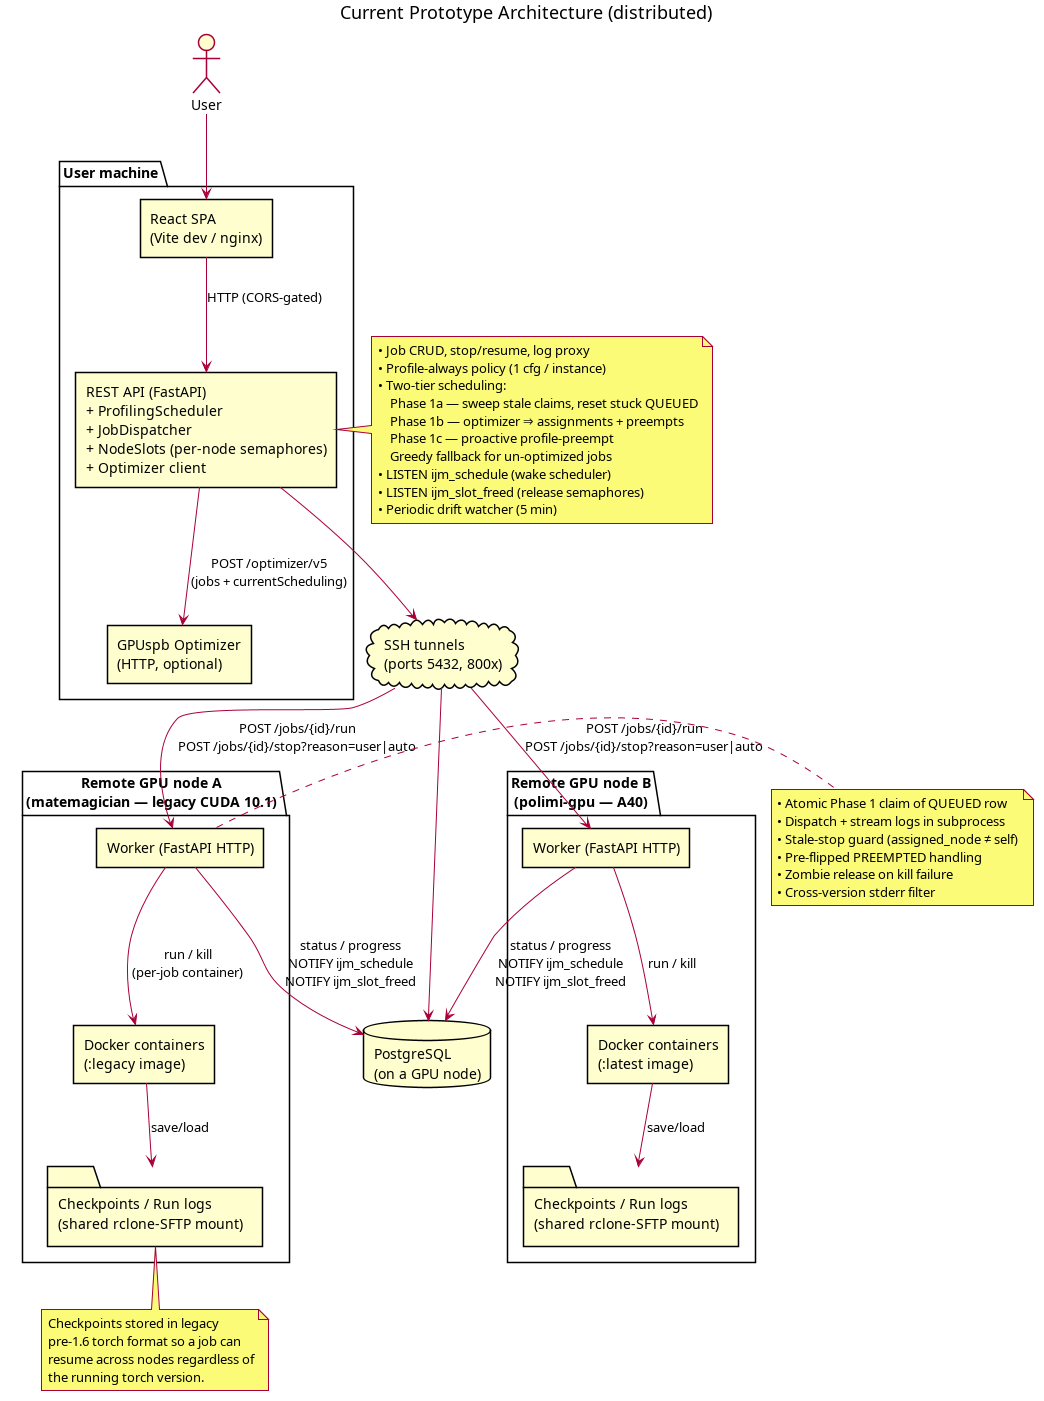
\includegraphics[width=\textwidth]{Images/CurrentPrototype.png}
\caption{Distributed prototype.  The~SPA, API, and~optimiser run on
the~operator's machine; workers and~Docker run on~each GPU node;
PostgreSQL runs on~a~GPU~node.  A~shared rclone-over-SFTP mount makes
checkpoints written by~one node visible from the~other.}
\label{fig:prototype}
\end{figure}

Single-process \texttt{docker compose} on~the~operator's machine is
supported for~development but is~not the~deployment target: any tradeoff
between local-dev simplicity and~distributed correctness resolves toward
the~distributed topology.

\section{Scheduling pipeline}\label{sec:sched-pipeline}

The pipeline is~shaped by~a~single governing assumption: \emph{profiling
is~always worth its cost}.  A~deep-learning job runs for~hours, whereas
profiling one GPU~configuration takes minutes; leaving a~configuration
unmeasured risks overlooking the~placement that~would have saved hours
of~computation, or~missing a~hard deadline.  The~scheduler therefore
treats profiling as~privileged work that~may preempt running jobs,
rather than as~best-effort measurement deferred until the~cluster falls
idle.  How~aggressively the~system profiles is~a~tunable policy:
\texttt{PROFILING\_CONFIGS\_PER\_JOB} (default~2) sets how~many
configurations each instance must measure before it~is~handed to~the
cost-aware optimiser for~standard placement.

A~single scheduling pass~--- \texttt{\_schedule\_waiting\_jobs} in
\texttt{app.py}~--- handles every dispatch decision.  It is~invoked
whenever a~job is~submitted, a~profiling run finishes, or~a~slot is
freed.  A~60-minute watchdog (\texttt{\_queue\_watcher}) serves as~a
safety net for~missed notifications, not as~the~main wake source.
Wake-ups are coalesced through a~single
\texttt{asyncio.Event} and~rate-limited to~at~most one pass every
five~seconds, so the~cluster has time to~apply the~previous plan before
the~next one is~computed.

The pass runs four phases, all guarded by~a~single
\texttt{schedule\_lock} except the~optimiser's HTTP call (phase~2),
which is~made outside the~lock so its timeout cannot stall concurrent
scheduler work:

\begin{enumerate}[leftmargin=*,itemsep=2pt,topsep=4pt]
  \item \textbf{Reset stuck assignments.}
    Reset \texttt{QUEUED} rows whose \texttt{assigned\_node} was set
    $\geq 30$~s ago without the~worker advancing them, so a~later phase
    can re-place the~row.
  \item \textbf{Optimiser pass.}
    Call the~optimiser outside the~lock (to~accommodate its 30~s HTTP
    timeout) and~apply its assignments through a~conditional
    \texttt{UPDATE \ldots WHERE assigned\_node IS NULL}, collecting the
    optimiser's preempt list.  The~optimiser only ever scores rows with
    \texttt{is\_profiling\_run = FALSE}~--- rows still owing a~profile
    run are invisible to~it.
  \item \textbf{Profile placement.}
    For~\texttt{QUEUED} rows that still owe a~profile run, the
    \texttt{ProfilingScheduler} atomically reserves the~instance's
    outstanding unmeasured \texttt{(node, GPU-count)} cells~--- up to~its
    \texttt{PROFILING\_CONFIGS\_PER\_JOB} budget (default~2)~--- and
    dispatches one of~them this pass, choosing the~node by~best fit
    on~remaining capacity; the~rest follow on~later passes as~slots
    free.  This is~the~mechanism behind the~\emph{profile-always}
    policy: an~instance must complete all~its profile runs before
    it~becomes a~candidate for~the optimiser-driven standard placement
    above.
  \item \textbf{Profile-preempt.}
    If~a~profile-owing row still has~no~slot after the~placement pass,
    find the~cheapest set of~low-priority \texttt{RUNNING} jobs whose
    eviction would free enough GPUs for~the~next unmeasured
    configuration.
\end{enumerate}

Once the~lock is~released, the~plan is~executed asynchronously: each
preempt and~each dispatch runs as~an~independent task, so a~slow stop
on~one node never delays placements on~another.  Before launching a~job,
the~dispatcher must acquire a~permit from the~destination node's
\texttt{NodeSlots} semaphore, whose count is~that node's GPU~capacity;
the~permit is~what bounds the~number of~concurrent jobs per~node and
arbitrates between tasks competing for~the~last free slot.

Permits are released asynchronously, because a~job's GPUs are not free
the~instant the~API decides to~stop it~--- only once the~worker has
killed the~container, drained its logs, and~written a~checkpoint.  The
worker therefore signals each release, and~the~API returns the~permit
at~that moment, keeping its in-memory count in~step with actual
occupancy.  Each release also records \emph{why} it~happened, because
the~cause determines whether the~scheduler should re-plan.  A~release
triggered by~an~event outside the~current plan~--- a~job finishing
on~its own, an~operator stopping a~job, or~the~cleanup of~an~orphaned
container~--- frees capacity the~optimiser did not foresee, and~so wakes
a~fresh scheduling pass.  A~release caused by~the~scheduler's \emph{own}
in-flight preempt is~the~one exception: the~plan that~issued the~preempt
already contains the~dispatch that~will reclaim the~freed slot, so
re-running the~optimiser at~that point would let it~rewrite a~plan it~is
still executing.  Only that case suppresses the~re-plan, and~doing so
is~safe because independent watchdogs~--- a~drift heartbeat, the
stuck-dispatch reaper, and~a~periodic queue watcher~--- re-wake the
scheduler if~a~planned dispatch ever fails to~land.

Figure~\ref{fig:seq-submit} shows the~submission path,
Figure~\ref{fig:seq-profiling-loop} the~cross-instance profile cycle,
Figure~\ref{fig:seq-optimizer-cycle} an~optimiser-driven preempt and
migrate round, and~Figure~\ref{fig:seq-standard-run} the~standard run.

\begin{figure}[H]
\centering
\footnotesize
\setlength{\unitlength}{0.7cm}
\resizebox{\textwidth}{!}{%
\begin{sequencediagram}
  \newthread{user}{User}
  \newinst[1.5]{api}{API}
  \newinst[1.5]{sched}{Scheduler}
  \newinst[1.5]{opt}{Optimizer}
  \newinst[1.5]{db}{PostgreSQL}
  \newinst[1.5]{worker}{Worker}

  \begin{call}{user}{\textsc{post} /jobs \{job\_id, dockerImage, \ldots\}}{api}{instance\_id}
    \begin{call}{api}{INSERT INTO jobs (status=QUEUED)}{db}{}
    \end{call}
    \begin{messcall}{api}{NOTIFY ijm\_schedule}{db}
    \end{messcall}
  \end{call}
  \begin{sdblock}{schedule pass}{coalesced, $\geq 5$s apart}
    \begin{call}{sched}{sweep stale claims; reset stuck QUEUED}{db}{}
    \end{call}
    \begin{call}{sched}{optimize(active jobs, currentScheduling)}{opt}{assignments, preempts}
    \end{call}
    \begin{call}{sched}{UPDATE assigned\_node WHERE NULL}{db}{}
    \end{call}
    \begin{callself}{sched}{profile-placement + profile-preempt scan}{}
    \end{callself}
    \begin{messcall}{sched}{dispatch\_with\_slot $\rightarrow$ acquire permit $\rightarrow$ POST /run}{worker}
    \end{messcall}
  \end{sdblock}
\end{sequencediagram}}
\caption{Submission and~scheduling.  The~API writes the~row and~notifies
the~scheduler; placement is~decided by~the~next pass.  The~optimiser
call sits outside the~schedule lock so its 30~s HTTP timeout cannot
block other passes.}
\label{fig:seq-submit}
\end{figure}

\begin{figure}[H]
\centering
\footnotesize
\setlength{\unitlength}{0.7cm}
\resizebox{\textwidth}{!}{%
\begin{sequencediagram}
  \newthread{worker}{Worker}
  \newinst[1.5]{docker}{Docker}
  \newinst[1.5]{sched}{Scheduler}
  \newinst[1.5]{db}{PostgreSQL}

  \begin{call}{worker}{atomic claim: UPDATE \ldots status=PROFILING}{db}{ok}
  \end{call}
  \begin{call}{worker}{docker run (profile container, isolated ckpt dir)}{docker}{exit code}
  \end{call}
  \begin{callself}{worker}{mean per-epoch duration (warmup epoch excluded)}{}
  \end{callself}
  \begin{call}{worker}{UPDATE profiling\_results SET duration\_seconds}{db}{}
  \end{call}
  \begin{call}{worker}{UPDATE jobs SET status=QUEUED, is\_profiling\_run=still\_owes}{db}{}
  \end{call}
  \begin{messcall}{worker}{NOTIFY ijm\_schedule}{db}
  \end{messcall}
  \begin{sdblock}{next scheduling pass}{}
    \begin{callself}{sched}{place this row as standard run, or pick next config to profile}{}
    \end{callself}
  \end{sdblock}
\end{sequencediagram}}
\caption{Profiling cycle.  Profile measurements are keyed by~the
(job-type, GPU-config) pair and~shared across submissions of~the~same
type.  Each instance profiles up~to~\texttt{PROFILING\_CONFIGS\_PER\_JOB}
(default~2) configurations before it~becomes a~standard-run candidate;
the~per-instance claim row guards against duplicate measurements.  The
worker records the~result and~re-queues the~row in~a~single transaction
(\texttt{worker/profiling.py:handle\_complete}).}
\label{fig:seq-profiling-loop}
\end{figure}

\begin{figure}[H]
\centering
\footnotesize
\setlength{\unitlength}{0.7cm}
\resizebox{\textwidth}{!}{%
\begin{sequencediagram}
  \newthread{sched}{Scheduler}
  \newinst[1.5]{opt}{Optimizer}
  \newinst[1.5]{db}{PostgreSQL}
  \newinst[1.5]{victim}{Worker (victim)}
  \newinst[1.5]{target}{Worker (target)}

  \begin{call}{sched}{POST /optimizer/v5 \{jobs, nodes, currentScheduling\}}{opt}{assignments + preempts}
  \end{call}
  \begin{callself}{sched}{stash pending\_migrates (in-memory)}{}
  \end{callself}
  \begin{messcall}{sched}{POST /stop?reason=auto}{victim}
  \end{messcall}
  \begin{call}{victim}{kill container, drain run task}{db}{}
    \begin{call}{victim}{UPDATE jobs SET status=QUEUED, assigned\_node=NULL}{db}{}
    \end{call}
    \begin{messcall}{victim}{NOTIFY ijm\_slot\_freed "node:n:auto\_preempt"}{db}
    \end{messcall}
  \end{call}
  \begin{callself}{sched}{release NodeSlots permit on LISTEN}{}
  \end{callself}
  \begin{call}{sched}{apply pending migrate on slot-freed LISTEN (\textsc{where} assigned\_node \textsc{is null})}{db}{}
  \end{call}
  \begin{messcall}{sched}{dispatch\_with\_slot $\rightarrow$ POST /run}{target}
  \end{messcall}
\end{sequencediagram}}
\caption{Optimiser-driven preempt and~migrate.  The~API trusts the
GPUspb plan: any job in~\texttt{currentScheduling} that the~optimiser
drops or~moves is~preempted with~\texttt{reason=auto}, clearing its
assignment.  Because an~\texttt{auto\_preempt} release deliberately does
\emph{not} wake a~fresh optimiser pass, a~moved job's new placement is
stashed in~\texttt{state.pending\_migrates} and~re-applied by~the~slot
listener (conditional \texttt{UPDATE \ldots WHERE assigned\_node IS
NULL}) once the~source \texttt{/stop} has drained the~row to
\textsc{queued}.}
\label{fig:seq-optimizer-cycle}
\end{figure}

\begin{figure}[H]
\centering
\footnotesize
\setlength{\unitlength}{0.7cm}
\resizebox{\textwidth}{!}{%
\begin{sequencediagram}
  \newthread{worker}{Worker}
  \newinst[1.5]{docker}{Docker}
  \newinst[1.5]{sched}{Scheduler}
  \newinst[1.5]{db}{PostgreSQL}

  \begin{call}{worker}{atomic claim: UPDATE \ldots status=RUNNING}{db}{ok}
  \end{call}
  \begin{call}{worker}{docker run (training container)}{docker}{exit code}
  \end{call}
  \begin{call}{worker}{UPDATE jobs SET SUCCEEDED/FAILED}{db}{}
  \end{call}
  \begin{messcall}{worker}{NOTIFY ijm\_slot\_freed "node:n:terminal"}{db}
  \end{messcall}
  \begin{sdblock}{next scheduling pass}{}
    \begin{callself}{sched}{place a waiting job on the freed slot}{}
    \end{callself}
  \end{sdblock}
\end{sequencediagram}}
\caption{Standard run.  The~worker performs an~atomic
conditional \texttt{UPDATE \ldots WHERE status = ANY(RUNNABLE\_STATUSES)}
so concurrent stops or~duplicate dispatches cannot race a~row into
\texttt{RUNNING}.  On~exit the~worker fires a~single
\texttt{ijm\_slot\_freed} (reason~\texttt{terminal}) in~the~same
transaction as~the~status flip; the~slot listener releases the~permit
and~wakes the~scheduler, so the~terminal path needs no~separate
\texttt{ijm\_schedule}.}
\label{fig:seq-standard-run}
\end{figure}

\section{Worker execution lifecycle}\label{sec:worker-lifecycle}

The scheduling pass decides \emph{where} a~job runs; the~worker's run
task (\texttt{\_run\_job}) owns \emph{how} it~runs and~how it~stops.  The
task moves through four phases (Table~\ref{tab:worker-phases}), and~every
database transition is~a~conditional \texttt{UPDATE}, so a~racing
\texttt{/stop}, the~stuck-dispatch reaper, or~a~duplicate dispatch cannot
corrupt the~row.

\begin{table}[H]
\centering\small
\begin{tabularx}{\textwidth}{@{}l >{\raggedright\arraybackslash}X >{\raggedright\arraybackslash}X@{}}
\toprule
\textbf{Phase} & \textbf{Action} & \textbf{Invariant it~enforces} \\
\midrule
1.~Claim    & Atomic \texttt{UPDATE \ldots status=RUNNING/PROFILING WHERE status} $\in$ \textsc{runnable} \texttt{AND assigned\_node=self} & A~\texttt{/stop} or~reaper that~already moved the~row makes the~claim miss, so no~container starts for~a~re-placed row. \\
2.~Launch   & Pick distinct physical GPU indices, prepare the~per-job checkpoint/runs directories, \texttt{docker run} & Distinct indices stop two 1-GPU jobs both landing on~GPU~0; an~in-process placeholder is~set \emph{before} any~\texttt{await}, so a~\texttt{/stop} cannot slip into the~window before the~container exists. \\
3.~Stream   & Parse \texttt{Epoch x/y} from~container stdout; flush the~latest value through a~once-per-second background writer & The~progress \texttt{UPDATE} is~conditional on~a~matching \texttt{status} and~\texttt{container\_name}, so a~reassigned row no-ops it~and~stops the~stream.  Coalescing replaces a~per-epoch round-trip that~fell behind over the~SSH-tunnelled connection. \\
4.~Complete & Write the~terminal status and~fire one~\texttt{ijm\_slot\_freed}; or, if~the~row was~migrated or~already stopped, record only the~exit code & A~kill-induced exit~137 never clobbers the~new owner's \textsc{running}; a~failed run also drops its~outstanding profile claims so their~cells are~not~left reserved. \\
\bottomrule
\end{tabularx}
\caption{The~worker run task's four phases~--- distinct from~the
scheduling pass's four phases above: that pass plans, this~task
executes.}\label{tab:worker-phases}
\end{table}

A~\texttt{/stop} and~its target run task are~separate coroutines that~must
not~race.  The~handler tags the~row in~an~in-process \texttt{stopping}
map, waits for~the~run task to~publish its~container
(\texttt{dispatch\_ready}), kills it, and~only \emph{after} awaiting the
run task's full drain writes the~final status and~frees the~slot
(Figure~\ref{fig:seq-worker-stop}).  The~run task's own completion phase,
seeing the~\texttt{stopping} tag, records just the~exit code, so the~slot
is~freed exactly once.  The~same hazard across nodes is~closed on~the~API
side: \texttt{dispatch\_with\_slot} awaits any in-flight \texttt{/stop}
on~the~target node before posting \texttt{/run}, so a~migration's new
container never starts before the~evicted one's CUDA context has~released
its~GPU.

\begin{figure}[H]
\centering
\footnotesize
\setlength{\unitlength}{0.7cm}
\resizebox{\textwidth}{!}{%
\begin{sequencediagram}
  \newthread{api}{API}
  \newinst[1.6]{run}{Worker run task}
  \newinst[1.6]{dock}{Docker}
  \newinst[1.6]{stop}{Worker /stop}
  \newinst[1.6]{db}{PostgreSQL}

  \begin{call}{api}{POST /run}{run}{202}
  \end{call}
  \begin{call}{run}{Phase 1: atomic claim status=RUNNING}{db}{ok}
  \end{call}
  \begin{call}{run}{Phase 2: docker run; set dispatch\_ready}{dock}{}
  \end{call}
  \begin{callself}{run}{Phase 3: stream stdout, progress @ 1/s}{}
  \end{callself}
  \begin{messcall}{api}{POST /stop?reason=auto  (stopping := auto)}{stop}
  \end{messcall}
  \begin{callself}{stop}{await dispatch\_ready}{}
  \end{callself}
  \begin{call}{stop}{kill container}{dock}{}
  \end{call}
  \begin{sdblock}{/stop awaits the run-task drain, then persists once}{}
    \begin{messcall}{dock}{exit 137}{run}
    \end{messcall}
    \begin{callself}{run}{Phase 4: stopping set $\Rightarrow$ record exit\_code only}{}
    \end{callself}
    \begin{call}{stop}{\_persist\_stop: status=QUEUED, assigned\_node=NULL}{db}{}
    \end{call}
    \begin{messcall}{stop}{NOTIFY ijm\_slot\_freed "node:n:auto\_preempt"}{db}
    \end{messcall}
  \end{sdblock}
\end{sequencediagram}}
\caption{Worker execution and~a~scheduler stop.  The~run task and~the
concurrent \texttt{/stop} synchronise through the~in-process
\texttt{dispatch\_ready} and~\texttt{stopping} maps plus a~drain await, so
the~slot is~freed exactly once and~by~exactly one path.  A
\texttt{reason=auto} stop returns the~row to~\textsc{queued} with~its
assignment cleared (a~\texttt{reason=user} stop lands on~\textsc{preempted}
instead); the~resulting \texttt{auto\_preempt} notify is~the~one the~slot
listener swallows (\S\ref{sec:sched-pipeline}).}
\label{fig:seq-worker-stop}
\end{figure}

\section{State machine}

Table~\ref{tab:state-machine} lists every transition a~job row can take.
All transitions are driven by~atomic conditional \texttt{UPDATE}s, so
concurrent stop, dispatch, and~completion paths cannot clobber each
other's work.

\begin{table}[H]
\centering\small
\begin{tabularx}{\textwidth}{@{}l l X@{}}
\toprule
\textbf{From} & \textbf{To} & \textbf{Trigger} \\
\midrule
\textsc{queued}     & \textsc{profiling} / \textsc{running} & Worker Phase~1 atomic claim \\
\textsc{profiling}  & \textsc{queued}     & Profile run finished; \texttt{is\_profiling\_run} flips to~\texttt{false} \\
\textsc{profiling}  & \textsc{failed}     & Profile container exited non-zero \\
\textsc{running}    & \textsc{succeeded} / \textsc{failed} & Container exit \\
\textsc{running}    & \textsc{preempted}  & User \texttt{POST /jobs/\{id\}/stop?reason=user} \\
\textsc{running}    & \textsc{queued}     & Scheduler preempt (\texttt{reason=auto}): clears \texttt{assigned\_node} for~the~next pass \\
\textsc{preempted} / \textsc{failed} & \textsc{queued} & \texttt{POST /jobs/\{id\}/resume} \\
\bottomrule
\end{tabularx}
\caption{Job state transitions.}\label{tab:state-machine}
\end{table}

Two distinct stop reasons separate \emph{user-initiated} preemption from
\emph{scheduler-initiated} preemption.  A~user stop is~sticky:
\textsc{preempted} stays put until the~user explicitly resumes.  A
scheduler stop returns the~row to~\textsc{queued} with~a~cleared
assignment, so the~next pass can place it~elsewhere automatically.  The
worker enforces this distinction and~ignores stale \texttt{/stop} calls
aimed at~a~row that has~since been re-assigned to~another node.

\section{Persistent state}\label{sec:persistent-state}

Two PostgreSQL tables hold every fact the~scheduler reads or~writes;
both are created idempotently on~startup from~\texttt{backend/schema.sql}.

\begin{lstlisting}[language=SQL, numbers=none]
CREATE TABLE jobs (
    id                  TEXT PRIMARY KEY,
    job_id              TEXT NOT NULL,
    image               TEXT NOT NULL,
    command             JSONB NOT NULL,
    script_path         TEXT,
    directory_to_mount  TEXT,
    status              TEXT NOT NULL,
    created_at          TIMESTAMPTZ NOT NULL,
    updated_at          TIMESTAMPTZ NOT NULL,
    container_name      TEXT,
    exit_code           INT,
    progress            TEXT,
    priority            INT DEFAULT 3,
    deadline            TIMESTAMPTZ,
    batch_size          INT,
    epochs_total        INT,
    profiling_epochs_no INT,
    assigned_node       TEXT,
    assigned_gpu_config JSONB,
    is_profiling_run    BOOLEAN DEFAULT FALSE
);

CREATE TABLE profiling_results (
    id               TEXT PRIMARY KEY,
    job_id           TEXT NOT NULL,
    instance_id      TEXT,
    gpu_config       JSONB NOT NULL,
    node_id          TEXT NOT NULL,
    duration_seconds FLOAT,
    created_at       TIMESTAMPTZ NOT NULL
);
\end{lstlisting}

Two columns of~\texttt{jobs} are load-bearing for~the~scheduling pass
above: \texttt{assigned\_node} is~the~target the~optimiser pass writes
under \texttt{WHERE assigned\_node IS NULL}, and~\texttt{is\_profiling\_run}
is~the~flag that makes a~row invisible to~the~optimiser (phase~2) and
visible to~the~\texttt{ProfilingScheduler} (phases~3--4).

A~unique index on~\texttt{(job\_id, gpu\_config)} makes the
cross-instance profile claim atomic.  Profile measurements are keyed
by~the~\emph{job type} (\texttt{job\_id}) and~the~GPU configuration, so
two concurrent submissions of~the~same type race to~own each unmeasured
cell; the~loser's INSERT trips the~unique constraint and~the~winner's
measurement is~shared by~every subsequent instance of~that type.

\section{Concurrency invariants}

The control plane relies on~three invariants, each defended in~code.

\textbf{No GPU oversubscription.}  Every dispatch goes through
\texttt{NodeSlots.acquire(node\_id,\,n\_gpus)}.  On~startup the
semaphores are reconciled from the~database: only rows in~\textsc{running}
or~\textsc{profiling} pre-acquire their permits, since a~\textsc{queued}
row with~an~assigned node has~no~live container yet (its dispatch task
acquires the~permit just before posting \texttt{/run}).  A~periodic drift
watcher recomputes the
authoritative count at~the~\texttt{IJM\_DRIFT\_HEARTBEAT\_S} cadence
(default 15~s) and~corrects any divergence.

\textbf{No duplicate containers per row.}  Both the~worker (Phase~1
claim, \texttt{running\_jobs[job\_id]} check) and~the~API
(\texttt{dispatch\_tasks[instance\_id]} deduplication) refuse a~second
concurrent dispatch for~the~same instance.  The~reaper that resets stuck
\textsc{queued} rows cancels any live dispatch task instead of
double-releasing its permit.

\textbf{Profiling is~sacred.}  Auto-preempt
(\texttt{\_preempt\_and\_release}) refuses to~act on
\texttt{is\_profiling\_run=TRUE}, and~profile-preempt (phase~4) filters
victims by~\texttt{status='RUNNING'} only.  Only an~explicit user stop
can cancel an~in-flight measurement.

\section{Stoppable, resumable, cross-node training}\label{sec:checkpoints}

A~job is~\emph{stoppable} because the~trainer persists its~state after
every epoch, and~\emph{resumable} because every (re)start loads that
state.  \texttt{BaseTrainer.train} writes \texttt{latest.pt} at~the~end
of~each epoch through a~temp-file-and-\texttt{rename}, so the~on-disk
checkpoint is~always a~whole epoch, never a~half-written file.  Stopping
a~job is~therefore just killing its~container
(\S\ref{sec:worker-lifecycle}): the~in-progress epoch is~discarded,
every completed epoch is~durable.  The~next dispatch~--- on~the~same node
or~another~--- reconstructs the~trainer, which loads \texttt{latest.pt},
restores the~model, optimiser, and~\texttt{current\_epoch}, and~continues
the~loop (Figure~\ref{fig:seq-resume}).  No~scheduler state mirrors
training progress; the~checkpoint file is~the~single source of~truth for
how far a~job has~run.

\begin{figure}[H]
\centering
\footnotesize
\setlength{\unitlength}{0.7cm}
\resizebox{0.85\textwidth}{!}{%
\begin{sequencediagram}
  \newthread{r1}{Trainer run --- node A}
  \newinst[2.4]{fs}{latest.pt (shared FS)}
  \newinst[2.4]{r2}{Trainer run --- node B}

  \begin{callself}{r1}{epoch $k$: train + evaluate}{}
  \end{callself}
  \begin{call}{r1}{atomic save (temp file $\rightarrow$ rename)}{fs}{}
  \end{call}
  \begin{callself}{r1}{epoch $k{+}1$: training\ldots\ container killed}{}
  \end{callself}
  \begin{call}{r2}{load $\Rightarrow$ epoch $k$, model + optimiser (strict=False)}{fs}{state}
  \end{call}
  \begin{callself}{r2}{resume from epoch $k{+}1$}{}
  \end{callself}
\end{sequencediagram}}
\caption{Stop and~resume.  The~trainer checkpoints after each epoch with
a~temp-file-and-\texttt{rename}, so \texttt{latest.pt} is~never
half-written.  A~stop kills the~container mid-epoch; the~next run~--- here
on~a~different node, possibly a~different torch version~--- loads
\texttt{latest.pt} and~continues.  Only the~interrupted epoch~$k{+}1$
is~recomputed.}
\label{fig:seq-resume}
\end{figure}

Two GPU generations coexist, so a~resume must survive a~change of~torch
version mid-job.  The~\texttt{matemagician} node is~pinned to~driver~418.x
(CUDA~10.1 max), so it~runs a~separate \texttt{:legacy} image built
on~PyTorch~1.5.1 and~Python~3.7; the~remaining nodes run the~default
\texttt{:latest} image on~PyTorch~2.6 and~CUDA~12.4.  Both images write
the~checkpoint in~the~legacy pre-1.6 \texttt{torch.save} format, and~the
load is~deliberately lenient: \texttt{strict=False} tolerates state-dict
key differences between versions, and~a~failed optimiser-state load
restarts Adam from~scratch rather than aborting the~resume~--- the~model
weights are~what matter, and~a~few epochs of~optimiser warmup are
invisible at~scenario timescales.  This is~what lets \texttt{cnn\_big}
migrate between a~modern A40 and~a~legacy P600 without losing progress.

The shared \texttt{data/} directory is~mounted on~every node via~rclone
over SFTP.  It~contains:

\begin{itemize}
  \item \texttt{data/checkpoints/\{job\_id\}/}~--- per-job checkpoints,
        mounted into the~container at~\texttt{/checkpoints};
  \item \texttt{data/runs/\{job\_id\}/}~--- captured stdout
        (\texttt{output.log}) and~TensorBoard artifacts, mounted at
        \texttt{/runs};
  \item \texttt{data/shared/data/}~--- read-only dataset cache (MNIST,
        CIFAR-10), mounted at~\texttt{/runs/data}.
\end{itemize}

Two worker-side environment variables let the~same
\texttt{nodes\_config.json} drive heterogeneous nodes.
\texttt{WORKER\_GPU\_MODE} selects how Docker exposes GPUs to~the
training container: \texttt{runtime} for~the~standard NVIDIA runtime,
\texttt{cdi} for~the~rootless daemon on~\texttt{polimi-gpu}, and
\texttt{none} for~a~CPU-only sandbox.  \texttt{IMAGE\_TAG\_OVERRIDE}
rewrites the~image tag, which is~how \texttt{matemagician} swaps
\texttt{:latest} for~\texttt{:legacy}.


\chapter{Configuration and Job Submission}\label{ch:config}
IJM is~configured at~three layers: a~pair of~JSON files that describe
the~cluster, an~HTTP submission API for~jobs, and~a~handful of~runtime
environment variables.  This section documents each in~turn.

\section{Cluster configuration}

The cluster topology is~loaded at~startup from two JSON files, whose
paths are configurable via~environment variables.

\subsection{Nodes (\texttt{nodes\_config.json})}

Each entry describes a~compute node and~its GPU resources.  The~example
below is~the~deployment used throughout
Chapter~\ref{ch:e2e}~(\texttt{config/nodes\_config.tunnel.json}); the
file checked in~at~\texttt{config/nodes\_config.json} is~a~mock cluster
used by~the~unit tests.

\begin{lstlisting}[language={}, numbers=none]
[
  {
    "id": "matemagician",
    "isForProfiling": true,
    "workerUrl": "http://localhost:8001",
    "cost": 0.10,
    "resources": [
      { "gpu_type": "QuadroP600", "gpu_count": 2 }
    ]
  },
  {
    "id": "polimi-gpu",
    "isForProfiling": true,
    "workerUrl": "http://localhost:8002",
    "cost": 0.30,
    "resources": [
      { "gpu_type": "A40", "gpu_count": 2 }
    ]
  }
]
\end{lstlisting}

\begin{table}[H]
\centering
\begin{tabularx}{\textwidth}{@{}l l X@{}}
\toprule
\textbf{Field} & \textbf{Type} & \textbf{Description} \\
\midrule
\texttt{id}                     & string         & Unique node identifier \\
\texttt{isForProfiling}         & bool           & If \texttt{true}, the~node can host profiling runs.  Production jobs may still land on~it; profiling jobs may only land on~it \\
\texttt{workerUrl}              & string         & HTTP base URL of~the~node's worker, reached through an~SSH tunnel.  The~API dispatches by~posting \texttt{/jobs/\{id\}/run} and~\texttt{/jobs/\{id\}/stop} here; every node must be~backed by~a~worker \\
\texttt{cost}                   & float          & Idle cost of~the~node ($\$$/h), used by~the~optimiser \\
\texttt{resources}              & array          & GPU resources attached to~the~node \\
\texttt{resources[].gpu\_type}  & string         & GPU model name (e.g.~\texttt{A40}, \texttt{L40S}, \texttt{QuadroP600}) \\
\texttt{resources[].gpu\_count} & int            & Number of~GPUs of~this type \\
\bottomrule
\end{tabularx}
\caption{Node configuration fields.}\label{tab:node-config}
\end{table}

GPU type and~count are declared explicitly rather than auto-detected.
This admits mixed-GPU nodes that ANDREAS did not support (e.g.~a~node
with~both A40 and~L40S GPUs), and~it~lets the~operator declare nodes
that are not physically attached to~the~API host~--- the~API only ever
talks to~workers over HTTP.

\subsection{Energy costs (\texttt{gpu\_energy\_costs.json})}

A~lookup table that maps a~GPU type and~bundle size to~an~hourly energy
cost (\$/h).  The~scheduler consults this table when scoring candidate
placements.

\begin{lstlisting}[language={}, numbers=none]
{
  "A40":        { "1": 0.30, "2": 0.55, "4": 1.05 },
  "L40S":       { "1": 0.40, "2": 0.75, "4": 1.40 },
  "QuadroP600": { "1": 0.03, "2": 0.055 },
  "Blackwell":  { "1": 1.00, "2": 1.85, "4": 3.50 }
}
\end{lstlisting}

\section{Job submission}

\textbf{Endpoint:} \texttt{POST /jobs}

\subsection{Request body}

\begin{lstlisting}[language={}, numbers=none]
{
  "job_id": "LSTM-small",
  "dockerImage": "ijm-lstm-small:dev",
  "scriptPath": "train.py",
  "directoryToMount": "/data/my-project",
  "Priority": 3,
  "deadline": "2026-03-20T18:00:00",
  "batchSize": 64,
  "profilingEpochsNo": 3,
  "epochsTotal": 20
}
\end{lstlisting}

\begin{table}[H]
\centering
\begin{tabularx}{\textwidth}{@{}l l l X@{}}
\toprule
\textbf{Field} & \textbf{Type} & \textbf{Required} & \textbf{Description} \\
\midrule
\texttt{job\_id}            & string       & yes & Reusable job type identifier; profile measurements are correlated across submissions sharing the~same \texttt{job\_id} \\
\texttt{dockerImage}        & string       & yes & Docker image to~execute \\
\texttt{scriptPath}         & string       & no  & Path to~the~training script (overrides Docker CMD with~\texttt{python3 <scriptPath>}) \\
\texttt{directoryToMount}   & string       & no  & Host directory persisted on~the~job row (ANDREAS-compatibility field); not~mounted by~the~current worker, which mounts only checkpoints, the~runs directory, and~the~shared dataset cache \\
\texttt{command}            & string[]     & no  & Command and~arguments (defaults to~the~image entrypoint; overridden by~\texttt{scriptPath}) \\
\texttt{Priority}           & int 1--5     & no  & Job priority (default~3) \\
\texttt{deadline}           & datetime     & no  & Job deadline (ISO 8601) \\
\texttt{batchSize}          & int          & no  & Batch size passed as~the~\texttt{BATCH\_SIZE} env var \\
\texttt{profilingEpochsNo}  & int $\geq 1$ & no  & Epochs per~profiling run (default~3) \\
\texttt{epochsTotal}        & int $\geq 1$ & no  & Total training epochs (default~20) \\
\bottomrule
\end{tabularx}
\caption{Job creation request fields.}\label{tab:job-create}
\end{table}

Each submission receives a~unique UUID instance ID (\texttt{id}) for
lifecycle tracking, separate from the~\texttt{job\_id} type identifier.
When \texttt{scriptPath} is~provided the~container runs
\texttt{python3 <scriptPath>}; otherwise the~image's default CMD is~used.
Unlike ANDREAS, \texttt{Priority} and~\texttt{deadline} are optional,
and~an~additional \texttt{command} field gives flexibility for
non-standard workloads.

\subsection{Response (201 Created)}

The response carries the~full job object, including the~scheduler's
initial decision: assigned node, GPU configuration, and~whether the
first run will be~a~profile or~a~standard execution.

\begin{lstlisting}[language={}, numbers=none]
{
  "id": "a1b2c3d4-...",
  "job_id": "LSTM-small",
  "image": "ijm-lstm-small:dev",
  "command": ["python3", "train.py"],
  "status": "QUEUED",
  "is_profiling_run": true,
  "assigned_node": "polimi-gpu",
  "assigned_gpu_config": { "A40": 1 },
  "priority": 3,
  "epochs_total": 20,
  "profiling_epochs_no": 3,
  "created_at": "2026-03-18T10:00:00Z",
  "updated_at": "2026-03-18T10:00:00Z",
  ...
}
\end{lstlisting}

\subsection{Job image requirements (the trainer contract)}
\label{sec:job-contract}

The fields above describe what the~API \emph{stores}; this subsection is~the
\emph{specification} a~container author implements so~a~job is~not~merely
runnable but~\emph{stoppable, resumable, and~migratable}.  A~job image is~a
container whose entrypoint instantiates a~subclass of~\texttt{BaseTrainer}
(\texttt{runtime/base.py}) and~calls \texttt{.train()}; subclassing \emph{is}
the~contract, and~in~return the~stop/resume/migrate machinery
of~\S\ref{sec:checkpoints} comes for~free.

\paragraph{What you implement.}  A~subclass provides up~to~three hooks
(Table~\ref{tab:trainer-hooks}).  For~a~dataset bundled with~the~runtime you
implement only \texttt{\_create\_model}: subclass one of~the~ready-made
mixins~--- \texttt{MNISTTrainer}, \texttt{MNISTSequenceTrainer}, or
\texttt{CIFAR10Trainer}~--- which already supply the~other two.

\begin{table}[H]
\centering\small
\begin{tabularx}{\textwidth}{@{}l >{\raggedright\arraybackslash}X@{}}
\toprule
\textbf{Hook (you override)} & \textbf{Signature and~contract} \\
\midrule
\texttt{\_create\_model}     & \texttt{(self) -> nn.Module}.  Return the~model.  \texttt{BaseTrainer} moves it~to~the~device and, on~a~multi-GPU node, wraps it~in~\texttt{nn.DataParallel} automatically. \\
\addlinespace
\texttt{\_load\_datasets}    & \texttt{(self) -> tuple[Dataset, Dataset]}.  Return \texttt{(train, test)} \emph{datasets}~--- not~\texttt{DataLoader}s; \texttt{BaseTrainer} builds the~loaders itself (train: \texttt{BATCH\_SIZE}, shuffled, \texttt{drop\_last}; test: \texttt{min(256, BATCH\_SIZE)}). \\
\addlinespace
\texttt{\_preprocess\_batch} & \texttt{(self, images, labels) -> tuple[Tensor, Tensor]}.  Reshape or~move a~batch before the~forward pass (e.g.\ \texttt{images.squeeze(1)} to~feed an~LSTM); return \texttt{(inputs, labels)}. \\
\bottomrule
\end{tabularx}
\caption{The~three trainer hooks.  With~a~bundled dataset only the~first
is~required~--- the~mixin supplies the~other two.}\label{tab:trainer-hooks}
\end{table}

\paragraph{What you get for~free.}  In~exchange for~honouring the~hooks,
\texttt{BaseTrainer} supplies the~behaviours the~scheduler relies
on~(Table~\ref{tab:job-contract}); the~mechanism behind each is~detailed
in~\S\ref{sec:checkpoints}.

\begin{table}[H]
\centering\small
\begin{tabularx}{\textwidth}{@{}l >{\raggedright\arraybackslash}X >{\raggedright\arraybackslash}X@{}}
\toprule
\textbf{The~image must\ldots} & \textbf{How \texttt{BaseTrainer} does it} & \textbf{Why IJM needs it} \\
\midrule
checkpoint after every epoch & writes \texttt{/checkpoints/latest.pt} via~a~temp-file-and-rename & the~checkpoint is~the~\emph{only} record of~progress, so a~job can~be~killed at~any~instant \\
resume on~start & loads \texttt{/checkpoints/latest.pt} (model, optimiser, epoch) before training & makes (re)dispatch idempotent: the~same image re-run on~another node continues rather than restarts \\
report progress on~stdout & logs \texttt{Epoch x/y - Loss: \ldots\ - Acc: \ldots\% - <s>s} once per~epoch & the~worker parses the~line for~live progress, and~the~trailing seconds is~the~per-epoch compute the~profiler records \\
take config from~the~environment & reads \texttt{EPOCHS\_TOTAL}, \texttt{BATCH\_SIZE} (and~\texttt{CHECKPOINT\_DIR}) & lets the~worker set the~epoch budget per~run~--- \texttt{profilingEpochsNo} for~a~profile, \texttt{epochsTotal} for~a~standard run \\
use all~assigned GPUs & wraps the~model in~\texttt{nn.DataParallel} across the~$N$ GPUs the~worker exposes & a~2-GPU placement only pays off if~the~job actually shards its~batch over both \\
tolerate \texttt{SIGKILL} & no~signal handler~--- a~kill just ends the~process & stopping a~job is~plain \texttt{docker kill}; safety comes from~the~epoch-boundary checkpoint, not~graceful shutdown \\
\bottomrule
\end{tabularx}
\caption{The~training-job contract.  An~image that~ignores it~still~\emph{runs},
but is~not~stoppable or~resumable: a~kill loses all~progress and~the~scheduler
cannot migrate it.}\label{tab:job-contract}
\end{table}

\paragraph{Scope of~the~built-in loop.}  The~supplied loop assumes
\emph{supervised single-label classification}: it~pairs an~\texttt{Adam}
optimiser ($\text{lr}=10^{-3}$) with~\texttt{CrossEntropyLoss}, feeds each
batch as~\texttt{(inputs, labels)}, and~scores top-1 accuracy.  A~workload that
fits this shape needs only the~hooks above.  One that~does~not~--- a~regression
target, a~custom loss, a~language-model objective~--- overrides \texttt{train}
or~\texttt{\_train\_one\_epoch} while still inheriting the~checkpoint and
progress contract, so it~stays stoppable and~resumable.  An~image that~bypasses
\texttt{BaseTrainer} altogether still runs, but~forfeits those guarantees.

\paragraph{A~complete job.}  The~following \texttt{train.py} is~a~full,
runnable IJM job in~its entirety~--- a~CNN on~CIFAR-10, using the~bundled
mixin so only \texttt{\_create\_model} is~written:

\begin{lstlisting}[language=Python, numbers=none]
# train.py
import torch.nn as nn
from base import CIFAR10Trainer        # bundled dataset mixin

class Net(nn.Module):
    def __init__(self, num_classes=10):
        super().__init__()
        self.body = nn.Sequential(
            nn.Conv2d(3, 32, 3, padding=1), nn.ReLU(),
            nn.AdaptiveAvgPool2d(1))
        self.head = nn.Linear(32, num_classes)

    def forward(self, x):
        return self.head(self.body(x).flatten(1))

class Trainer(CIFAR10Trainer):         # data + batch wiring inherited
    def _create_model(self) -> nn.Module:
        return Net()

if __name__ == "__main__":
    Trainer().train()   # stop/resume/progress: automatic
\end{lstlisting}

\paragraph{Packaging and~runtime inputs.}  The~image bundles \texttt{base.py}
beside the~script and~runs it~as~the~entrypoint:

\begin{lstlisting}[language={}, numbers=none]
FROM python:3.13-slim
RUN pip install torch torchvision
COPY base.py train.py ./
CMD ["python", "-u", "train.py"]
\end{lstlisting}

At~dispatch the~worker sets \texttt{EPOCHS\_TOTAL} and~\texttt{BATCH\_SIZE}
(a~profile run passes \texttt{profilingEpochsNo} as~\texttt{EPOCHS\_TOTAL},
Table~\ref{tab:job-create}) and~bind-mounts the~per-job checkpoint directory
at~the~default \texttt{CHECKPOINT\_DIR}\,=\,\texttt{/checkpoints}.
The~legacy P600 node, pinned to~CUDA~10.1 / PyTorch~1.5.1, is~served by~a
parallel \texttt{Dockerfile.legacy} selected through \texttt{IMAGE\_TAG\_OVERRIDE}
(\S\ref{sec:checkpoints}); the~only constraint this~adds is~that~the~trainer
module must \emph{import} under Python~3.7.

\paragraph{Datasets.}  The~bundled mixins fetch MNIST and~CIFAR-10 into~the
shared cache at~\texttt{/runs/data} (Table~\ref{tab:shared-fs}), staged once
and~mounted read-only on~every node.  A~custom dataset must currently be~baked
into~the~image or~added to~that~shared cache: the~\texttt{directoryToMount}
submission field is~retained for~ANDREAS compatibility but~is~not~bind-mounted
by~the~present worker.

\section{Full API overview}

Table~\ref{tab:api-endpoints} lists every endpoint.  Interactive
documentation is~available at~\texttt{/docs} (Swagger~UI) and
\texttt{/redoc} when the~API is~running.

\begin{table}[H]
\centering
\begin{tabularx}{\textwidth}{@{}l l X@{}}
\toprule
\textbf{Method} & \textbf{Path} & \textbf{Description} \\
\midrule
\texttt{GET}    & \texttt{/}                            & Health check endpoint \\
\texttt{GET}    & \texttt{/health}                      & Detailed health check~--- pings DB and~checks job runner \\
\texttt{GET}    & \texttt{/nodes}                       & List all~cluster nodes with~their current status \\
\texttt{GET}    & \texttt{/gpu-costs}                   & Hourly GPU energy costs used by~the~scheduler for~optimisation \\
\texttt{GET}    & \texttt{/configurations}              & List all~valid hardware configurations in~the~cluster \\
\texttt{POST}   & \texttt{/jobs}                        & Create a~new job \\
\texttt{GET}    & \texttt{/jobs}                        & List all~jobs ordered by~creation time (paginated via \texttt{limit}/\texttt{offset}) \\
\texttt{GET}    & \texttt{/jobs/\{id\}}                 & Get a~specific job by~ID \\
\texttt{POST}   & \texttt{/jobs/\{id\}/stop}            & Request job to~be stopped (user-driven; sticky \textsc{preempted} state) \\
\texttt{POST}   & \texttt{/jobs/\{id\}/resume}          & Request job to~be resumed \\
\texttt{DELETE} & \texttt{/jobs/\{id\}}                 & Delete a~job, killing any~running container first \\
\texttt{DELETE} & \texttt{/jobs}                        & Delete all~jobs and~their profiling results \\
\texttt{GET}    & \texttt{/jobs/\{id\}/logs}            & Return the~output log for~a~job by~proxying to~the~worker that~owns it \\
\texttt{GET}    & \texttt{/profiling-results/\{id\}}    & All~profiling results for~a~job, ordered by~duration (fastest first) \\
\texttt{GET}    & \texttt{/admin/slots}                 & NodeSlots snapshot: in-memory \texttt{used} vs.\ DB-authoritative count \\
\texttt{POST}   & \texttt{/admin/reconcile-slots}       & Force NodeSlots to~match DB-authoritative state (idempotent) \\
\texttt{GET}    & \texttt{/admin/dispatch-tasks}        & List in-flight \texttt{\_dispatch\_when\_slot\_free} tasks \\
\bottomrule
\end{tabularx}
\caption{API endpoints.}\label{tab:api-endpoints}
\end{table}

Three architectural choices set IJM's control plane apart from ANDREAS.
First, the~\emph{job-management} logic~--- scheduling, profiling, and~dispatch~---
is~consolidated into a~single FastAPI service, where ANDREAS used a~separate
Java Jobs Manager.  The~cost-aware optimiser itself is~\emph{not}
reimplemented: IJM consumes the~GPUspb
solver~\cite{filippini2023pathrelinking,filippini2024stochastic}~--- the~same
line of~work as~ANDREAS's optimiser~--- as~an~external service, so what~is
consolidated is~the~job manager, not~the~optimiser.
Second, execution lives in~per-node \emph{workers}~--- also FastAPI~---
that the~API reaches over HTTP through SSH tunnels; that same GPUspb
optimiser is~reached the~same way and~owns every standard-run placement
decision.
Third, IJM exposes explicit \texttt{stop}, \texttt{resume},
\texttt{logs}, and~\texttt{delete} endpoints, together with
\texttt{/profiling-results} and~\texttt{/configurations}, so the~user
has direct visibility into the~scheduler's state.

\section{Runtime environment}

Table~\ref{tab:env-vars} lists the~runtime knobs that influence the
scheduler.  Unless noted otherwise, every variable is~read by~the~API
process at~startup.

\begin{table}[H]
\centering
\begin{tabularx}{\textwidth}{@{}l l X@{}}
\toprule
\textbf{Variable} & \textbf{Default} & \textbf{Description} \\
\midrule
\texttt{DATABASE\_URL}                  & \texttt{postgresql://\ldots/ijm} & PostgreSQL DSN, reached via~SSH tunnel \\
\texttt{OPTIMIZER\_URL}                 & unset & The~GPUspb HTTP service used for~standard-run placement \\
\texttt{OPTIMIZER\_METHOD}              & \texttt{RG} & GPUspb solver method passed in~the~request body \\
\texttt{OPTIMIZER\_VERBOSE}             & 0 & Per-call log verbosity (0--3) \\
\texttt{PROFILING\_CONFIGS\_PER\_JOB}   & 2 & How many distinct GPU configurations a~single instance profiles before falling through to~a~standard run \\
\texttt{IJM\_DRIFT\_HEARTBEAT\_S}       & 15 & Period of~the~slot-tracker drift heartbeat that reconciles the~in-memory slot count against the~database-authoritative count per~node \\
\texttt{WORKER\_GPU\_MODE}              & \texttt{runtime} & Worker-side; how Docker exposes GPUs to~training containers (\texttt{runtime} / \texttt{cdi} / \texttt{none}) \\
\texttt{IMAGE\_TAG\_OVERRIDE}           & unset & Worker-side; rewrites \texttt{:latest} to~the~given tag.  Used on~\texttt{matemagician} to~pick the~CUDA-10.1-compatible \texttt{:legacy} image \\
\texttt{HOST\_ROOT}, \texttt{HOST\_PROJECT\_ROOT} & \texttt{/host} & Resolve container-internal vs.~host paths for~Docker bind mounts; \texttt{HOST\_PROJECT\_ROOT} falls back to \texttt{HOST\_ROOT} when unset \\
\bottomrule
\end{tabularx}
\caption{Key environment variables.}\label{tab:env-vars}
\end{table}


\chapter{End-to-End Scenarios}\label{ch:e2e}
\subsection{Objective and cost model}
\label{sec:e2e-objective}

The scheduler minimises
\[
\textsc{TotalCost} \;=\; \sum_{j} \texttt{GPUcost}(j) + \sum_{j} \texttt{TardWeight}(j) \cdot \max\bigl(0, \texttt{finish}(j) - \texttt{deadline}(j)\bigr),
\]
where \texttt{GPUcost} is wall-clock time times the bundle hourly rate
(Table~\ref{tab:e2e-rates}, left) and \texttt{TardWeight} grows with
job priority (Table~\ref{tab:e2e-rates}, right).  With slack deadlines
the cheapest plan wins; under deadline pressure the tardiness term
shifts urgent jobs onto the fastest available bundle.

\begin{table}[h!]\centering\small
\begin{tabular}{lr}\toprule
GPU bundle & \$/hour \\\midrule
\texttt{QuadroP600$\times$1} & 0.030 \\
\texttt{QuadroP600$\times$2} & 0.055 \\
\texttt{A40$\times$1}        & 0.300 \\
\texttt{A40$\times$2}        & 0.550 \\\bottomrule
\end{tabular}
\quad
\begin{tabular}{cc}\toprule
Priority & TardWeight (\$/sec) \\\midrule
1 & 0.000254 \\
4 & 0.000396 \\
5 & 0.000444 \\\bottomrule
\end{tabular}
\caption{Bundle hourly rates and per-priority tardiness weights.  Two-GPU
bundles include a small co-location discount.}\label{tab:e2e-rates}
\end{table}

\paragraph{Cluster.}  Two profiling-capable nodes, four slots total:

\begin{center}\small
\begin{tabular}{l l l}\toprule
Node              & GPUs                  & Bundle hourly cost \\\midrule
\texttt{matemagician}\,(n1) & 2$\times$\texttt{QuadroP600} & 0.055 \\
\texttt{polimi-gpu}\,(n2)   & 2$\times$\texttt{A40}        & 0.550 \\\bottomrule
\end{tabular}
\end{center}

For each new job type the profile sweep exercises all four
\texttt{(node, GPU-count)} cells (\texttt{configs\_per\_job}{=}2, four
instances).

% ---------------------------------------------------------------------------
\subsection{Two-GPU placement}
\label{sec:e2e-multi-gpu}

The \texttt{cnn\_big} workload (ten $3{\times}3$ conv blocks,
$3{\to}64{\to}128{\to}256{\to}384{\to}512$ channels,
$128{\times}128{\times}3$ inputs, batch $32$) is sized so per-step
compute amortises DataParallel sync overhead on both GPU classes.
Table~\ref{tab:e2e-2gpu} reports per-epoch wall-clock times from the
profile sweep (\texttt{SelectJobs\_times.csv}).

\begin{table}[h!]\centering\small
\begin{tabular}{l r r r}\toprule
Bundle & per-epoch [s] & rel.\ 1-GPU & GPUcost/epoch [\$] \\\midrule
\texttt{A40$\times$1}        & 6.294  & --                                  & 0.000525 \\
\texttt{A40$\times$2}        & \textbf{5.626} & \textbf{1.12$\times$ faster} & 0.000859 \\
\texttt{QuadroP600$\times$1} & 51.064 & --                                  & 0.000426 \\
\texttt{QuadroP600$\times$2} & \textbf{30.322} & \textbf{1.68$\times$ faster} & 0.000463 \\\bottomrule
\end{tabular}
\caption{Measured per-epoch wall-clock and GPUcost for
\texttt{cnn\_big}; both 2-GPU bundles beat their 1-GPU
sibling.}\label{tab:e2e-2gpu}
\end{table}

Over $40$ epochs the four plans cost \$0.0210, \$0.0344, \$0.0170,
\$0.0185 (A40$\times$1, A40$\times$2, P600$\times$1, P600$\times$2
respectively).  P600$\times$1 is the cost-minimum for slack
deadlines.  P600$\times$2 is only \$0.0015 more expensive but $41\%$
faster, so any deadline that P600$\times$1 misses by more than
$3.4$\,s at priority~5 flips the ranking to P600$\times$2; this is
the cell exercised in Scenario~2 Stage~3.

% ---------------------------------------------------------------------------
\subsection{Scenario 1 --- single type}
\label{sec:e2e-s1}

\begin{table}[h!]\centering\small
\begin{tabular}{l l r l l}\toprule
Label & Type & Priority & Deadline & Submitted at \\\midrule
JOB1 & \texttt{lstm-small} & 4 & $+1$\,h    & $t=0$\,s    \\
JOB2 & \texttt{lstm-small} & 4 & $+1$\,h    & $t=5$\,s    \\
JOB3 & \texttt{lstm-small} & 4 & $+1$\,h    & $t=10$\,s   \\
JOB4 & \texttt{lstm-small} & 4 & $+1$\,h    & $t=15$\,s   \\
URGENT$^{\star}$ & \texttt{lstm-small} & 5 & $+90$\,s & end of S1 \\\bottomrule
\end{tabular}
\caption{Scenario~1 submissions.}\label{tab:e2e-s1-jobs}
\end{table}

\begin{figure}[h!]\centering
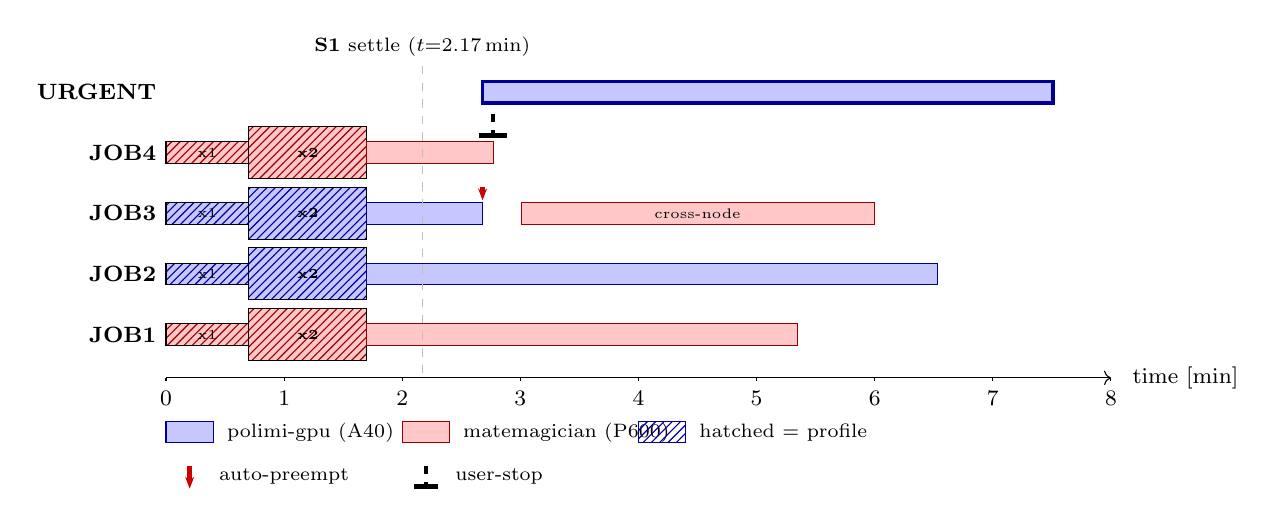
\begin{tikzpicture}[x=1.5cm, y=0.55cm, font=\footnotesize,
    nodeA40/.style={draw=blue!60!black, fill=blue!22, line width=0.4pt},
    nodeP600/.style={draw=red!60!black,  fill=red!22,  line width=0.4pt},
    profhatchA/.style={pattern=north east lines, pattern color=blue!60!black},
    profhatchP/.style={pattern=north east lines, pattern color=red!60!black},
  ]
  % v9 measured run, scenario start 2026-05-12 22:37:51.
  % Stage events (min): S1 settle 2.17, URGENT placed 2.68, user-stop 2.77,
  % resume verified 3.01, drain done 14.07.
  % Bars: 2-GPU profile cell is drawn TALLER than 1-GPU to give 2-GPU
  % its own visual signal (caption explains).
  \draw[->] (0,0) -- (8.0,0);
  \foreach \t in {0,1,2,3,4,5,6,7,8} \draw (\t,0) -- (\t,-0.08) node[below] {\t};
  \node[anchor=west] at (8.1,0) {time [min]};

  % JOB1 (P600 red): profile-x1 0--0.7, profile-x2 0.7--1.7 (TALLER), standard 1.7--5.35.
  \node[anchor=east] at (0,1) {\textbf{JOB1}};
  \draw[nodeP600] (0,0.75) rectangle (0.7,1.25);
    \draw[profhatchP] (0,0.75) rectangle (0.7,1.25); \node at (0.35,1) {\tiny x1};
  \draw[nodeP600] (0.7,0.4) rectangle (1.7,1.6);
    \draw[profhatchP] (0.7,0.4) rectangle (1.7,1.6); \node at (1.2,1) {\tiny\textbf{x2}};
  \draw[nodeP600] (1.7,0.75) rectangle (5.35,1.25);

  % JOB2 (A40 blue): profile-x1 0--0.7, profile-x2 0.7--1.7, standard 1.7--6.53.
  \node[anchor=east] at (0,2.4) {\textbf{JOB2}};
  \draw[nodeA40] (0,2.15) rectangle (0.7,2.65);
    \draw[profhatchA] (0,2.15) rectangle (0.7,2.65); \node at (0.35,2.4) {\tiny x1};
  \draw[nodeA40] (0.7,1.8) rectangle (1.7,3.0);
    \draw[profhatchA] (0.7,1.8) rectangle (1.7,3.0); \node at (1.2,2.4) {\tiny\textbf{x2}};
  \draw[nodeA40] (1.7,2.15) rectangle (6.53,2.65);

  % JOB3 (A40 blue then P600 red cross-node):
  \node[anchor=east] at (0,3.8) {\textbf{JOB3}};
  \draw[nodeA40] (0,3.55) rectangle (0.7,4.05);
    \draw[profhatchA] (0,3.55) rectangle (0.7,4.05); \node at (0.35,3.8) {\tiny x1};
  \draw[nodeA40] (0.7,3.2) rectangle (1.7,4.4);
    \draw[profhatchA] (0.7,3.2) rectangle (1.7,4.4); \node at (1.2,3.8) {\tiny\textbf{x2}};
  \draw[nodeA40] (1.7,3.55) rectangle (2.68,4.05);
  \draw[ultra thick, red!80!black, -{Stealth[length=1.5mm]}] (2.68,4.4) -- (2.68,4.1);
  \draw[nodeP600] (3.01,3.55) rectangle (6.0,4.05);
  \node at (4.5,3.8) {\tiny cross-node};

  % JOB4 (P600 red, user-stopped):
  \node[anchor=east] at (0,5.2) {\textbf{JOB4}};
  \draw[nodeP600] (0,4.95) rectangle (0.7,5.45);
    \draw[profhatchP] (0,4.95) rectangle (0.7,5.45); \node at (0.35,5.2) {\tiny x1};
  \draw[nodeP600] (0.7,4.6) rectangle (1.7,5.8);
    \draw[profhatchP] (0.7,4.6) rectangle (1.7,5.8); \node at (1.2,5.2) {\tiny\textbf{x2}};
  \draw[nodeP600] (1.7,4.95) rectangle (2.77,5.45);
  \draw[ultra thick, black, dashed, -{Bar[width=3.5mm]}] (2.77,6.1) -- (2.77,5.55);

  % URGENT (A40 blue): standard 2.68--7.51, thicker border.
  \node[anchor=east] at (0,6.6) {\textbf{URGENT}};
  \draw[nodeA40, line width=1.2pt] (2.68,6.35) rectangle (7.51,6.85);

  % Only ONE stage marker — S1 settle.  Other event timestamps marked
  % inline by the preempt-arrow / user-stop-bar.
  \draw[dashed,gray!50] (2.17,7.2) -- (2.17,0);
  \node[anchor=south] at (2.17,7.2) {\scriptsize \textbf{S1} settle ($t{=}2.17$\,min)};

  % Two-row legend below: row 1 = node colours + profile hatch;
  % row 2 = event markers.  Generous horizontal spacing to avoid overlap.
  \begin{scope}[shift={(0,-1.5)}, x=1.0cm, y=0.45cm]
    \draw[nodeA40] (0,0) rectangle (0.6,0.6);
    \node[anchor=west] at (0.65,0.3) {\scriptsize polimi-gpu (A40)};
    \draw[nodeP600] (3.0,0) rectangle (3.6,0.6);
    \node[anchor=west] at (3.65,0.3) {\scriptsize matemagician (P600)};
    \draw[nodeA40, profhatchA] (6.0,0) rectangle (6.6,0.6);
    \node[anchor=west] at (6.65,0.3) {\scriptsize hatched $=$ profile};
  \end{scope}
  \begin{scope}[shift={(0,-2.6)}, x=1.0cm, y=0.45cm]
    \draw[ultra thick, red!80!black, -{Stealth[length=1.5mm]}] (0.3,0.7) -- (0.3,0.05);
    \node[anchor=west] at (0.55,0.4) {\scriptsize auto-preempt};
    \draw[ultra thick, black, dashed, -{Bar[width=3mm]}] (3.3,0.7) -- (3.3,0.05);
    \node[anchor=west] at (3.55,0.4) {\scriptsize user-stop};
  \end{scope}
\end{tikzpicture}
\caption{Scenario~1 timeline (v9, 2026-05-12).  Taller bars in the
profile phase are the 2-GPU profile cells.  Slot count $\leq 2$ on
each node at every instant.}\label{fig:e2e-s1}
\end{figure}

Four patient \texttt{lstm-small} jobs plus one \texttt{URGENT}
(Table~\ref{tab:e2e-s1-jobs}).  Table~\ref{tab:e2e-s1-opt} gives the
per-bundle ExecTime and GPUcost the optimiser saw at the S1 round.

\begin{table}[h!]\centering\small
\begin{tabular}{l r r r r}\toprule
Bundle & per-epoch [s] & GPUcost/epoch [\$] & 40-ep cost [\$] & Rank \\\midrule
A40$\times$1        & 7.25  & 0.000604  & 0.0242  & --- \\
A40$\times$2        & 9.12  & 0.001393  & 0.0557  & worst \\
QuadroP600$\times$1 & 5.47  & 0.0000456 & 0.00182 & \textbf{best} \\
QuadroP600$\times$2 & 10.66 & 0.000163  & 0.00651 & --- \\\bottomrule
\end{tabular}
\caption{Per-bundle cost the optimiser sees at the S1 round; slack
deadlines so TardCost$=0$.}\label{tab:e2e-s1-opt}
\end{table}

Settled placement: JOB1, JOB2 $\to$ \texttt{polimi-gpu} A40$\times$1
(overflow); JOB3, JOB4 $\to$ \texttt{matemagician} P600$\times$1.  At
S2 the URGENT comparison (Table~\ref{tab:e2e-s1-urgent}) chooses
A40$\times$1, evicting JOB2.

\begin{table}[h!]\centering\scriptsize
\begin{tabular}{l r r r r r l}\toprule
Plan for URGENT      & ExecTime [s] & GPUcost [\$] & Tardiness [s] & TardCost [\$] & TotalCost [\$] & Decision \\\midrule
A40$\times$1 (preempt JOB2) & 217 & 0.0181 & 127 & 0.0564 & \textbf{0.0745} & \checkmark\ chosen \\
P600$\times$1 (no preempt)  & 442 & 0.0037 & 352 & 0.1563 & 0.1600          & rejected \\\bottomrule
\end{tabular}
\caption{Optimiser plan comparison for URGENT at the S2
round.}\label{tab:e2e-s1-urgent}
\end{table}

\paragraph{Measured run (\texttt{v9}).}
S1 settles at $t{=}2.17$\,min with all four profile cells exercised
($\{$A40$\times$1, A40$\times$2, P600$\times$1, P600$\times$2$\}$).
URGENT (\texttt{7d7c848a}) placed in $6$\,s; auto-preempt victim
JOB3 (\texttt{0f6f54c4} on \texttt{polimi-gpu}).  Operator user-stops
JOB4 (\texttt{c957097f}; sticky \texttt{PREEMPTED}).  JOB3 resumes
from checkpoint within the $10$-minute Stage~4 budget.  Terminal at
$t{=}14.07$\,min: $4$ \texttt{SUCCEEDED}, $1$ \texttt{PREEMPTED},
$0$ \texttt{FAILED}.  Slot tracker: \texttt{acquire\_oversub\_count}$=0$,
\texttt{release\_underflow\_count}$=1$,
\texttt{drift\_recovery\_count}$=60$.


% ---------------------------------------------------------------------------
\subsection{Scenario 2 --- two types}
\label{sec:e2e-s2}

\begin{table}[h!]\centering\small
\begin{tabular}{l l r l}\toprule
Label & Type & Priority & Deadline \\\midrule
JOB1 & S (\texttt{lstm-small}) & 1 & $+8$\,h \\
JOB2 & B (\texttt{cnn\_big})   & 1 & $+8$\,h \\
JOB3 & S (\texttt{lstm-small}) & 4 & $+1$\,h \\
JOB4 & B (\texttt{cnn\_big})   & 4 & $+2$\,h \\
URG-S$^{\star}$ (S2) & S & 5 & $+90$\,s \\
URG-B$^{\star}$ (S3) & B & 5 & $+90$\,s \\
JOB7 (S4.5) & opposite of user-stop victim & 1 & $+8$\,h \\\bottomrule
\end{tabular}
\caption{Scenario~2 submissions.}\label{tab:e2e-s2-jobs}
\end{table}

\begin{figure}[h!]\centering
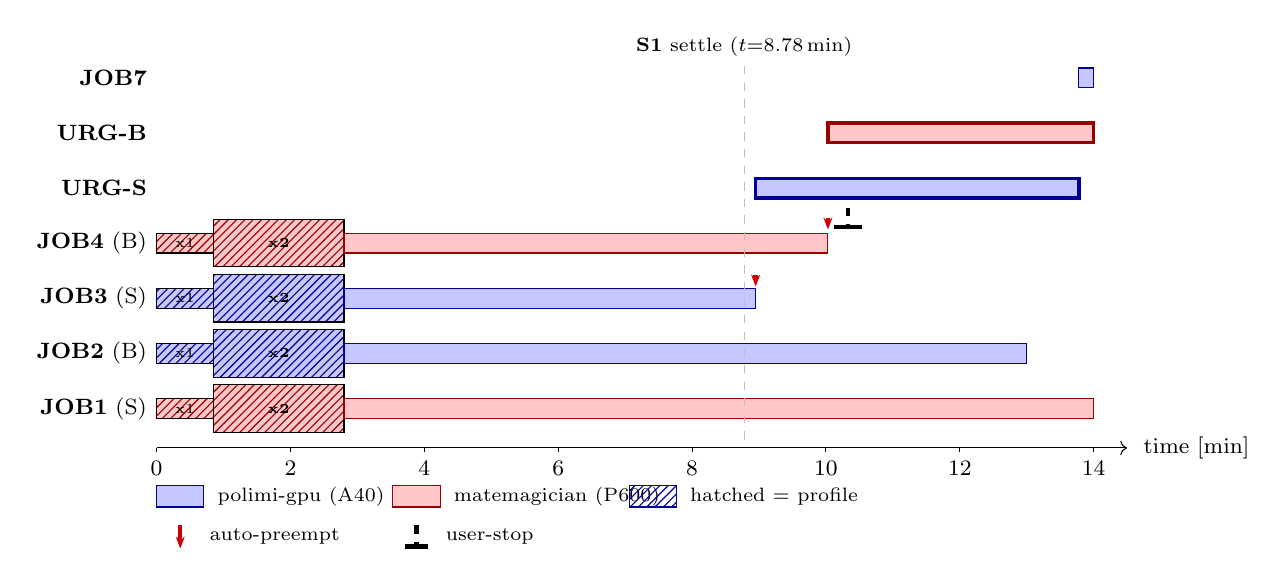
\begin{tikzpicture}[x=0.85cm, y=0.50cm, font=\footnotesize,
    nodeA40/.style={draw=blue!60!black, fill=blue!22, line width=0.4pt},
    nodeP600/.style={draw=red!60!black,  fill=red!22,  line width=0.4pt},
    profhatchA/.style={pattern=north east lines, pattern color=blue!60!black},
    profhatchP/.style={pattern=north east lines, pattern color=red!60!black},
  ]
  % Timestamps are anchored to the v14 measured run (scenario start at
  % 11:35:11).  Stage events: S1 settle 8.78\,min, URG-S placed 8.95,
  % URG-B placed 10.03, user-stop 10.33, JOB7 submit 10.38.
  \draw[->] (0,0) -- (14.5,0);
  \foreach \t in {0,2,4,6,8,10,12,14} \draw (\t,0) -- (\t,-0.1) node[below] {\t};
  \node[anchor=west] at (14.6,0) {time [min]};

  % JOB1 (S, P600 red): profile x1 + x2 (taller x2), standard 2.8--end.
  \node[anchor=east] at (0,1) {\textbf{JOB1} (S)};
  \draw[nodeP600] (0,0.75) rectangle (0.85,1.25);
    \draw[profhatchP] (0,0.75) rectangle (0.85,1.25); \node at (0.425,1) {\tiny x1};
  \draw[nodeP600] (0.85,0.4) rectangle (2.8,1.6);
    \draw[profhatchP] (0.85,0.4) rectangle (2.8,1.6); \node at (1.825,1) {\tiny\textbf{x2}};
  \draw[nodeP600] (2.8,0.75) rectangle (14.0,1.25);

  % JOB2 (B, A40 blue): profile x1 + x2, standard 2.8--13.
  \node[anchor=east] at (0,2.4) {\textbf{JOB2} (B)};
  \draw[nodeA40] (0,2.15) rectangle (0.85,2.65);
    \draw[profhatchA] (0,2.15) rectangle (0.85,2.65); \node at (0.425,2.4) {\tiny x1};
  \draw[nodeA40] (0.85,1.8) rectangle (2.8,3.0);
    \draw[profhatchA] (0.85,1.8) rectangle (2.8,3.0); \node at (1.825,2.4) {\tiny\textbf{x2}};
  \draw[nodeA40] (2.8,2.15) rectangle (13.0,2.65);

  % JOB3 (S, A40 blue): profile + brief standard, preempted at S2.
  \node[anchor=east] at (0,3.8) {\textbf{JOB3} (S)};
  \draw[nodeA40] (0,3.55) rectangle (0.85,4.05);
    \draw[profhatchA] (0,3.55) rectangle (0.85,4.05); \node at (0.425,3.8) {\tiny x1};
  \draw[nodeA40] (0.85,3.2) rectangle (2.8,4.4);
    \draw[profhatchA] (0.85,3.2) rectangle (2.8,4.4); \node at (1.825,3.8) {\tiny\textbf{x2}};
  \draw[nodeA40] (2.8,3.55) rectangle (8.95,4.05);
  \draw[ultra thick, red!80!black, -{Stealth[length=1.5mm]}] (8.95,4.4) -- (8.95,4.1);

  % JOB4 (B, P600 red): profile + standard, preempted at S3, user-stopped at S4.5.
  \node[anchor=east] at (0,5.2) {\textbf{JOB4} (B)};
  \draw[nodeP600] (0,4.95) rectangle (0.85,5.45);
    \draw[profhatchP] (0,4.95) rectangle (0.85,5.45); \node at (0.425,5.2) {\tiny x1};
  \draw[nodeP600] (0.85,4.6) rectangle (2.8,5.8);
    \draw[profhatchP] (0.85,4.6) rectangle (2.8,5.8); \node at (1.825,5.2) {\tiny\textbf{x2}};
  \draw[nodeP600] (2.8,4.95) rectangle (10.03,5.45);
  \draw[ultra thick, red!80!black, -{Stealth[length=1.5mm]}] (10.03,5.85) -- (10.03,5.55);
  \draw[ultra thick, black, dashed, -{Bar[width=3.5mm]}] (10.33,6.1) -- (10.33,5.55);

  % URG-S (S, A40 blue): 8.95 to 13.78 (lstm-small A40 4.83 min).
  \node[anchor=east] at (0,6.6) {\textbf{URG-S}};
  \draw[nodeA40, line width=1.2pt] (8.95,6.35) rectangle (13.78,6.85);

  % URG-B (B, P600 red): 10.03 to chart end.
  \node[anchor=east] at (0,8.0) {\textbf{URG-B}};
  \draw[nodeP600, line width=1.2pt] (10.03,7.75) rectangle (14.0,8.25);

  % JOB7 (S, A40 blue): submitted at 10.38, dispatched at 13.78 once
  % URG-S vacates.  Bar starts at dispatch — no dotted "queued" line
  % (it added noise without conveying info).
  \node[anchor=east] at (0,9.4) {\textbf{JOB7}};
  \draw[nodeA40] (13.78,9.15) rectangle (14.0,9.65);

  % Single stage marker at S1 settle.
  \draw[dashed,gray!50] (8.78,9.7) -- (8.78,0);
  \node[anchor=south] at (8.78,9.7) {\scriptsize \textbf{S1} settle ($t{=}8.78$\,min)};

  % Two-row legend below.
  \begin{scope}[shift={(0,-1.5)}, x=1.0cm, y=0.45cm]
    \draw[nodeA40] (0,0) rectangle (0.6,0.6);
    \node[anchor=west] at (0.65,0.3) {\scriptsize polimi-gpu (A40)};
    \draw[nodeP600] (3.0,0) rectangle (3.6,0.6);
    \node[anchor=west] at (3.65,0.3) {\scriptsize matemagician (P600)};
    \draw[nodeA40, profhatchA] (6.0,0) rectangle (6.6,0.6);
    \node[anchor=west] at (6.65,0.3) {\scriptsize hatched $=$ profile};
  \end{scope}
  \begin{scope}[shift={(0,-2.6)}, x=1.0cm, y=0.45cm]
    \draw[ultra thick, red!80!black, -{Stealth[length=1.5mm]}] (0.3,0.7) -- (0.3,0.05);
    \node[anchor=west] at (0.55,0.4) {\scriptsize auto-preempt};
    \draw[ultra thick, black, dashed, -{Bar[width=3mm]}] (3.3,0.7) -- (3.3,0.05);
    \node[anchor=west] at (3.55,0.4) {\scriptsize user-stop};
  \end{scope}
\end{tikzpicture}
\caption{Scenario~2 timeline (v14, 2026-05-13).  Taller bars are the
2-GPU profile cells.  URG-S preempts JOB3 at $t{=}8.95$\,min; URG-B
preempts JOB4 at $t{=}10.03$; user-stop on JOB4 at $t{=}10.33$; JOB7
queued at $t{=}10.38$ (dotted) and dispatched once URG-S vacates A40
at $t{=}13.78$.}\label{fig:e2e-s2}
\end{figure}

Submissions in Table~\ref{tab:e2e-s2-jobs}: four patient jobs split
across two types, two back-to-back URGENT submissions at S2/S3, and a
late JOB7 at S4.5.

\begin{table}[h!]\centering\small
\begin{tabular}{l l r r r r}\toprule
Type & Bundle & per-epoch [s] & 40-epoch [s] & rate [\$/h] & 40-ep cost [\$] \\\midrule
S & A40$\times$1        & 7.25  & 290  & 0.300 & 0.0242 \\
S & A40$\times$2        & 9.12  & 365  & 0.550 & 0.0557 \\
S & QuadroP600$\times$1 & 5.47  & 219  & 0.030 & 0.00182 \\
S & QuadroP600$\times$2 & 10.66 & 426  & 0.055 & 0.00651 \\\midrule
B & A40$\times$1        & 6.29  & 252  & 0.300 & 0.0210 \\
B & \textbf{A40$\times$2}        & \textbf{5.63}  & \textbf{225}  & 0.550 & 0.0344 \\
B & QuadroP600$\times$1 & 51.06 & 2042 & 0.030 & 0.0170 \\
B & \textbf{QuadroP600$\times$2} & \textbf{30.32} & \textbf{1213} & 0.055 & \textbf{0.0185} \\\bottomrule
\end{tabular}
\caption{Per-bundle profile data the optimiser sees at the S1
round.}\label{tab:e2e-s2-opt}
\end{table}

\paragraph{Settled S1 placement.}
JOB1, JOB3 (lstm-small) $\to$ \texttt{matemagician} P600$\times$1;
JOB2, JOB4 (cnn\_big) $\to$ \texttt{polimi-gpu} A40$\times$1.  The
overflow ranking is by ``cost lost if forced off the cheap node'':
lstm-small loses \$0.0224, cnn\_big loses \$0.0040, so lstm-small
keeps both P600 slots.  Total \$0.0456.

\paragraph{URGENT plans at S2 and S3.}

\begin{table}[h!]\centering\scriptsize\setlength{\tabcolsep}{3pt}
\begin{tabular}{l l r r r r r l}\toprule
URGENT & Plan & ExecTime [s] & GPUcost [\$] & Tard [s] & TardCost [\$] & Total [\$] & Decision \\\midrule
URG-S & QuadroP600$\times$1 (preempt JOB1)            & 219  & 0.00182 & 109  & 0.0484 & \textbf{0.0502} & \checkmark\ chosen \\
URG-S & A40$\times$1 (preempt JOB2)                   & 290  & 0.0242  & 180  & 0.0799 & 0.1041          & rejected \\\midrule
URG-B & A40$\times$1 (preempt JOB2)                   & 252  & 0.0210  & 162  & 0.0719 & \textbf{0.0929} & \checkmark\ chosen \\
URG-B & A40$\times$2 (preempt JOB2+JOB4)              & 225  & 0.0344  & 135  & 0.0599 & 0.0943          & 2nd ($\Delta 1.5\%$) \\
URG-B & QuadroP600$\times$2 (preempt JOB1+JOB3)       & 1213 & 0.0185  & 1123 & 0.4986 & 0.517           & 3rd \\
URG-B & QuadroP600$\times$1 (preempt JOB1 or JOB3)    & 2042 & 0.0170  & 1952 & 0.8667 & 0.884           & 4th \\\bottomrule
\end{tabular}
\caption{Optimiser plan comparison for URG-S (S2) and URG-B
(S3).}\label{tab:e2e-s2-urgent}
\end{table}

\paragraph{Measured run (\texttt{v14}).}
S1 settles at $t{=}8.78$\,min with profile coverage $4{\times}2=8$
cells.  URG-S (\texttt{8d875cc9}) placed in $17$\,s; auto-preempt
victim JOB3 (\texttt{d47acbf3}, lstm-small on \texttt{polimi-gpu}).
URG-B (\texttt{5e9b9820}) placed in $24$\,s; auto-preempt victim
JOB4 (\texttt{9658d9df}, cnn\_big on \texttt{matemagician}).  Stage~4
verifies $\geq 1$ cross-node resume: JOB3 receives
\texttt{assigned\_node=matemagician} (cross-node from its
\texttt{polimi-gpu} origin); JOB4 resumes on its origin
\texttt{matemagician}.  Operator user-stops JOB4 at $t{=}10.33$\,min;
late JOB7 (\texttt{fd074cb2}) submitted at $t{=}10.38$\,min and
backfills polimi-gpu A40 once URG-S vacates ($t{=}13.78$\,min).


% ---------------------------------------------------------------------------
\subsection{Reproducibility}

Every numerical entry in Tables~\ref{tab:e2e-2gpu},
\ref{tab:e2e-s1-opt}, \ref{tab:e2e-s1-urgent}, \ref{tab:e2e-s2-opt}
and~\ref{tab:e2e-s2-urgent} is taken verbatim from the optimiser's
per-round inputs (\texttt{Lof\_Selectjobs.csv},
\texttt{SelectJobs\_times.csv}, \texttt{GPU-costs.csv}) and chosen
plan (\texttt{results/RG\_schedule\_*.csv}) under
\texttt{<optimizer>/calls/call\_<ts>.0/}.  The two scenarios are
driven by \texttt{infra/e2e\_scenario.sh} and
\texttt{infra/e2e\_scenario\_2types.sh}, both of which print one line
per assertion and expose the slot tracker via
\texttt{GET /admin/slots}.


\chapter{Conclusion}\label{ch:conclusion}
\section{Summary of contributions}

IJM extends the~ANDREAS prototype from a~single-host scheduler into
a~distributed control plane: one FastAPI service drives per-node
workers over SSH-tunnelled HTTP, and~an~external GPUspb optimiser is
consumed as~a~peer service rather than embedded in~the~scheduler.  On
top of~that topology the~report names three substantive
contributions.  A~\emph{profile-always} policy keyed by~the~unique
index on~\texttt{(job\_id, gpu\_config)}~--- so~that profile
measurements are atomically shared across instances of~the~same job
type.  \emph{Cross-version checkpoint resume} between
PyTorch~1.5.1 (CUDA~10.1, \texttt{matemagician}) and~PyTorch~2.6
(CUDA~12.4, \texttt{polimi-gpu}), enabling an~in-flight job to~migrate
between heterogeneous GPU generations without losing progress.  And
an~empirical characterisation of~the~horizon-myopia in~GPUspb's
\texttt{method=RG} proxy (Chapter~\ref{ch:e2e}), traced through both
scenarios to~three combining mechanics: horizon-myopic tardiness,
\texttt{Heuristic::assign}'s refusal to~displace incumbents, and~the
``cheapest if~deadline reachable, else fastest'' fallback.

\section{Limitations}

The reference deployment uses GPUspb's \texttt{method=RG}, whose proxy
is~horizon-myopic; the~deadline-aware \texttt{method=PR} variant
exists upstream but is~not the~default and~has not been validated end
to~end against the~IJM control plane.  The~report contains
no~baseline-algorithm comparison~--- IJM's behaviour is~documented
against the~true objective, but not yet against FIFO, EDF, or
priority-only baselines on~the~same workloads.  Worker-side coverage
is~end-to-end only (\texttt{worker/tests/} is~empty); only two GPU
generations (A40 and~QuadroP600) have been validated; and~the~cluster
used throughout Chapter~\ref{ch:e2e} is~two nodes with~four GPU slots
in~total, so the~scaling properties of~the~four-phase pass at~tens
of~nodes are an~open question.

\section{Future work}

Two follow-ups have concrete entry points in~the~codebase.  First,
re-run Scenarios~1 and~2 with
\texttt{OPTIMIZER\_METHOD=PR}: \texttt{proxy\_function\_max} is~per-job
deadline-aware, so the~prediction from~\S\ref{sec:e2e-s1-urgent-math}
is~that URGENT lands on~A40$\times$2 in~round~1 rather than migrating
into it~over two patient-completion events.  Second, extend the
two-node evaluation to~a~larger cluster once a~third GPU class is
available; this is~where the~profile-claim's atomicity and~the
optimiser-call latency (currently a~30~s timeout) will be~stressed.


\nocite{andreas}
\bibliographystyle{alpha}
\bibliography{main}
\addcontentsline{toc}{chapter}{Bibliography}

\end{document}
